\section{MapReduce}
\label{ssec:mapreduce}

En las secciones anteriores, se habló de Procesamiento Paralelo y Distribuido,
se mencionaron algunas características (particularmente las más afínes a este
documento), en esta sección, se busca aplicar las cuestiones que se mencionaron
con anterioridad, y empezamos a hablar del núcleo del documento
\textit{MapReduce}.

MapReduce (\acrshort{mr}), es un modelo de programación; una forma de hacer las cosas; un
paradigma. Este modelo fue introducido por Google en la primer mitad del
2000~\cite{dean2004} y la implementación del mismo se asocia con grandes 
\glspl{dataset} y es
aplicable a una gran cantidad de tareas del mundo real~\cite{dean2008}. En esta
sección se avanza sobre una introducción acerca del modelo que presenta
MapReduce y 
luego se aplicarán los conceptos en una de las varias herramientas que aplican
el modelo en cuestion, la herramienta a la que se hacer referencia es un 
\Gls{framework} para Big Data, su nombre es 
\textit{Hadoop}
\includegraphics[height=10pt]{figuras/logos/hadoop_logo.png}.

\subsection{Funciones \texttt{Map} y \texttt{Reduce}}

\paragraph{Un vistazo general:}
en este modelo los usuarios que implementan \acrshort{mr} definen dos
funciones principales, una función \textit{Map} y una función \textit{Reduce},
el sistema que da soporte a la aplicación implementada se encarga de
paralelizar la ejecución de la misma a lo largo y ancho de un sistema
distribuido (\gls{cluster}) de ordenadores, este \gls{cluster} cuenta con las
características de los sistemas distribuidos mencionados en la sección
\ref{sec:procesamiento_distribuido}. Sistemas como estos permiten que Google
(en el 2008) pueda procesar 20\acrshort{pb} por día~\cite{dean2008}.

Las implementaciones de diferentes cargas de trabajo llevadas a cabo en el 
2004 por Google con este nuevo modelo de programación sentaba sus bases sobre un
desarrollo anterior extremadamente importante, el Sistema de Archivos de
Google (\acrshort{gfs}, por sus siglas en inglés)~\cite{ghemawat2003}, el cual,
en resumidas cuentas, es un sistema de archivos distribuidos (lo cual está en
línea con lo presentado anteriormente con respecto a la ``paralelización de datos'').

\subsubsection{Map}
\label{sssec:map}

\paragraph{Resumen} Esta función {\tt map}, se distribuye automáticamente sobre el sistema
distribuido, y puede trabajar ya sobre {\it chunks} (partición) de datos
que se encuentran dentro de los diferentes nodos, a los cuales se les distribuye el
procesamiento de dicha función. 

\begin{figure}[h!]
  \centering
  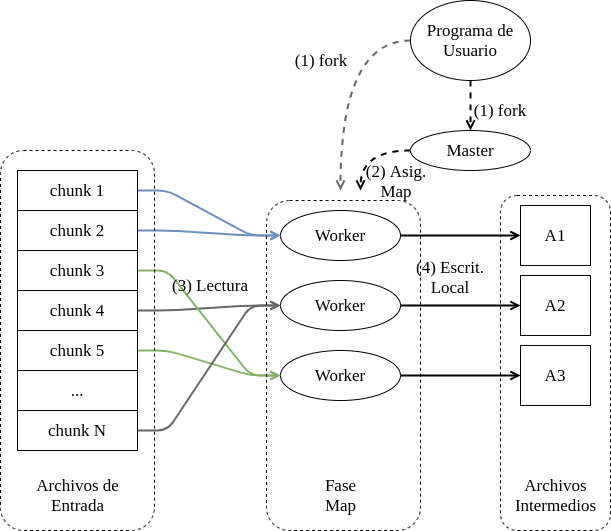
\includegraphics[width=0.75\linewidth]{figuras/MapReduce_mapper_phase.png}
  \caption{MapReduce: Fase {\tt map}}
  \label{fig:mapreduce_mapper_phase}
\end{figure}



\begin{enumerate}
\item {\bf fork:} El sistema distribuido se encarga de realizar la replicación
      de la aplicación del usuario sobre el conjunto de máquinas, esta
      aplicación se divide en copias que son {\it workers} y una especial que
      se denomina {\it master}\footnote{Esto es análogo a lo que se estudia en
      la cátedra con OpenMPI.}. Este último es el encargado de dividir las
      tareas a las copias que son workers.
\item {\bf Asig. Map:} El {\it master} asigna las tareas a los workers. Los
      cuales, cabe aclarar, trabajan sobre un o varios chunks de datos locales al
      nodo.
\item {\bf Lectura:} Un {\it worker} al que se le asigna una tarea {\tt map},
      lee los contenidos de los {\it archivos de entrada}, interpreta estos
      datos en formato clave-valor y se encarga de distribuir estos pares a la
      función {map}. Los valores que se produzcan por la función {\it map}, 
      se almacenan en un buffer de memoria.
\item {\bf Escritura Local:} Periodicamente, los pares que se almacenan en el
      buffer de memoria, pasan a ser escritos al disco de manera particionada. Las 
      ubicaciones de las particiones se comunican al {\it master} el cual será
      responsable más adelante de distribuir esta info. a los {\it workers} que
      son parte del {\it reduce}.
\end{enumerate}

\subsubsection{Reduce}
\label{sssec:reduce}


